


\begin{figure*}
\begin{minipage}{\textwidth}
	\begin{minipage}[b]{0.5\textwidth}
		\setlength\tabcolsep{4pt}
		\begin{tabular}{lcc}
			\toprule
			Split & \# of games (in $10^3$) & \# of moves (in $10^6$)\\ %
			\midrule
			Train-S & 	\phantom{1}15 	& \phantom{1}1.1\\ %
			Train-M & 	\phantom{1}50 	& \phantom{1}3.7\\ %
			Train-L & 	200 			& 15.0\\ 			 %
			Dev 	& 	\phantom{1}15 	& \phantom{1}1.1\\ %
			Test 	& 	\phantom{1}15 	& \phantom{1}1.1\\ %
			\bottomrule
		\end{tabular}
		\captionof{table}{Statistics of the language modeling data.}
		\label{tab:data_stats}
	\end{minipage}
	\hfill
	\begin{minipage}[b]{0.48\textwidth}
		\centering
		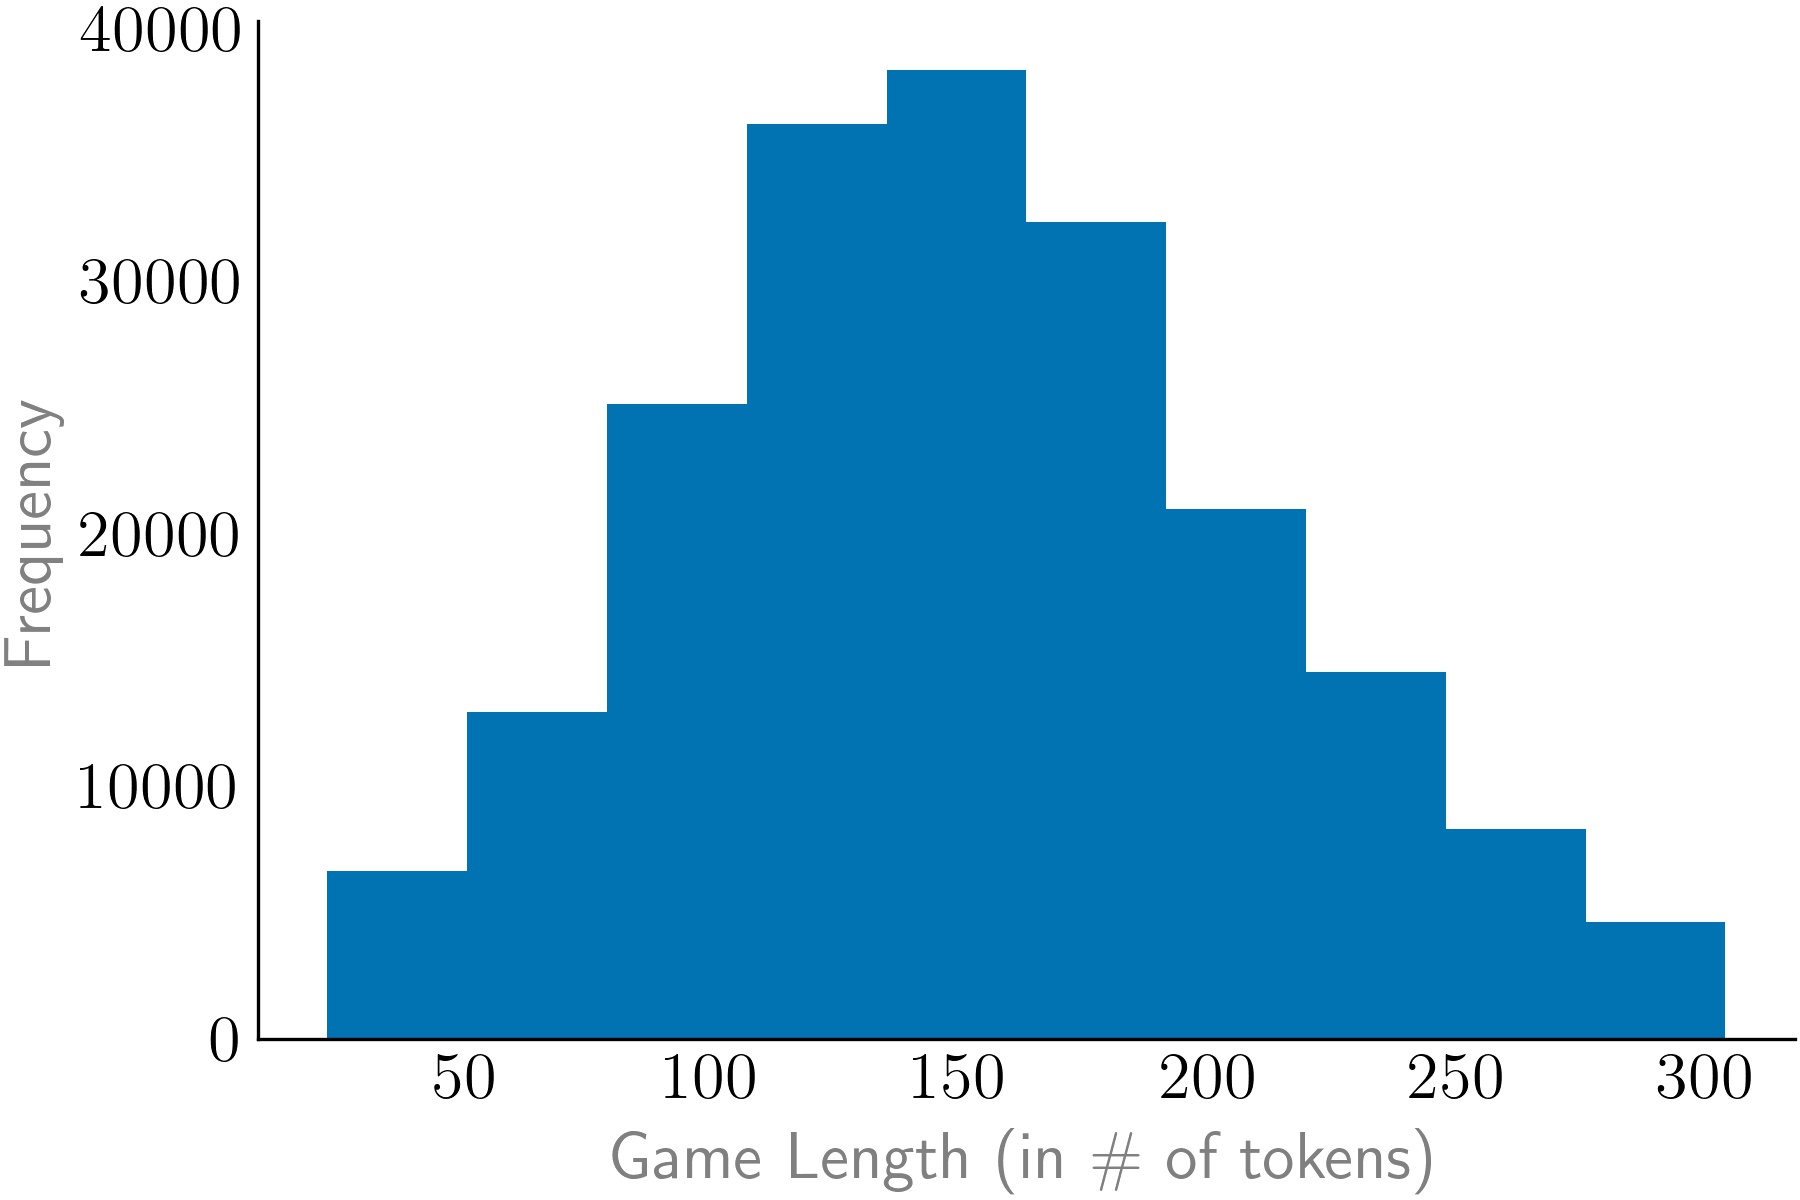
\includegraphics[width=0.8\textwidth]{figures/hist_game}
		\vspace{-0.1in}
		\captionof{figure}{Histogram of tokenized game lengths for Train-L.}
		\label{fig:hist_len}
	\end{minipage}
\end{minipage}
\end{figure*}


\begin{figure*}
	\begin{minipage}{\textwidth}
		\begin{minipage}[b]{0.48\textwidth}
			\centering
			\setlength\tabcolsep{4pt}
			\begin{tabular}{lccc}
				\toprule
				Piece type & End/Start-Actual & End-Other & Start-Other\\ %
				\midrule
				Rook (\pos{R}) & 	358 	& 273     & 197\\ 
				Knight (\pos{N}) & 	144 	& 136 & 126\\  
				Bishop (\pos{B}) & 	164 			& 170 & 161\\
				Queen (\pos{Q}) 	& 	204 	& 103  & 129 \\ 
				
				King (\pos{K}) & 	130 	& 318  & 387\\
				\midrule
				Total & 1000 & 1000 & 1000 \\\bottomrule
			\end{tabular}
			\captionof{table}{Piece type counts for ending square prediction prompts.}
			\label{tab:probe_data_stats}
		\end{minipage}
		\hfill
		\begin{minipage}[b]{0.48\textwidth}
			\centering
			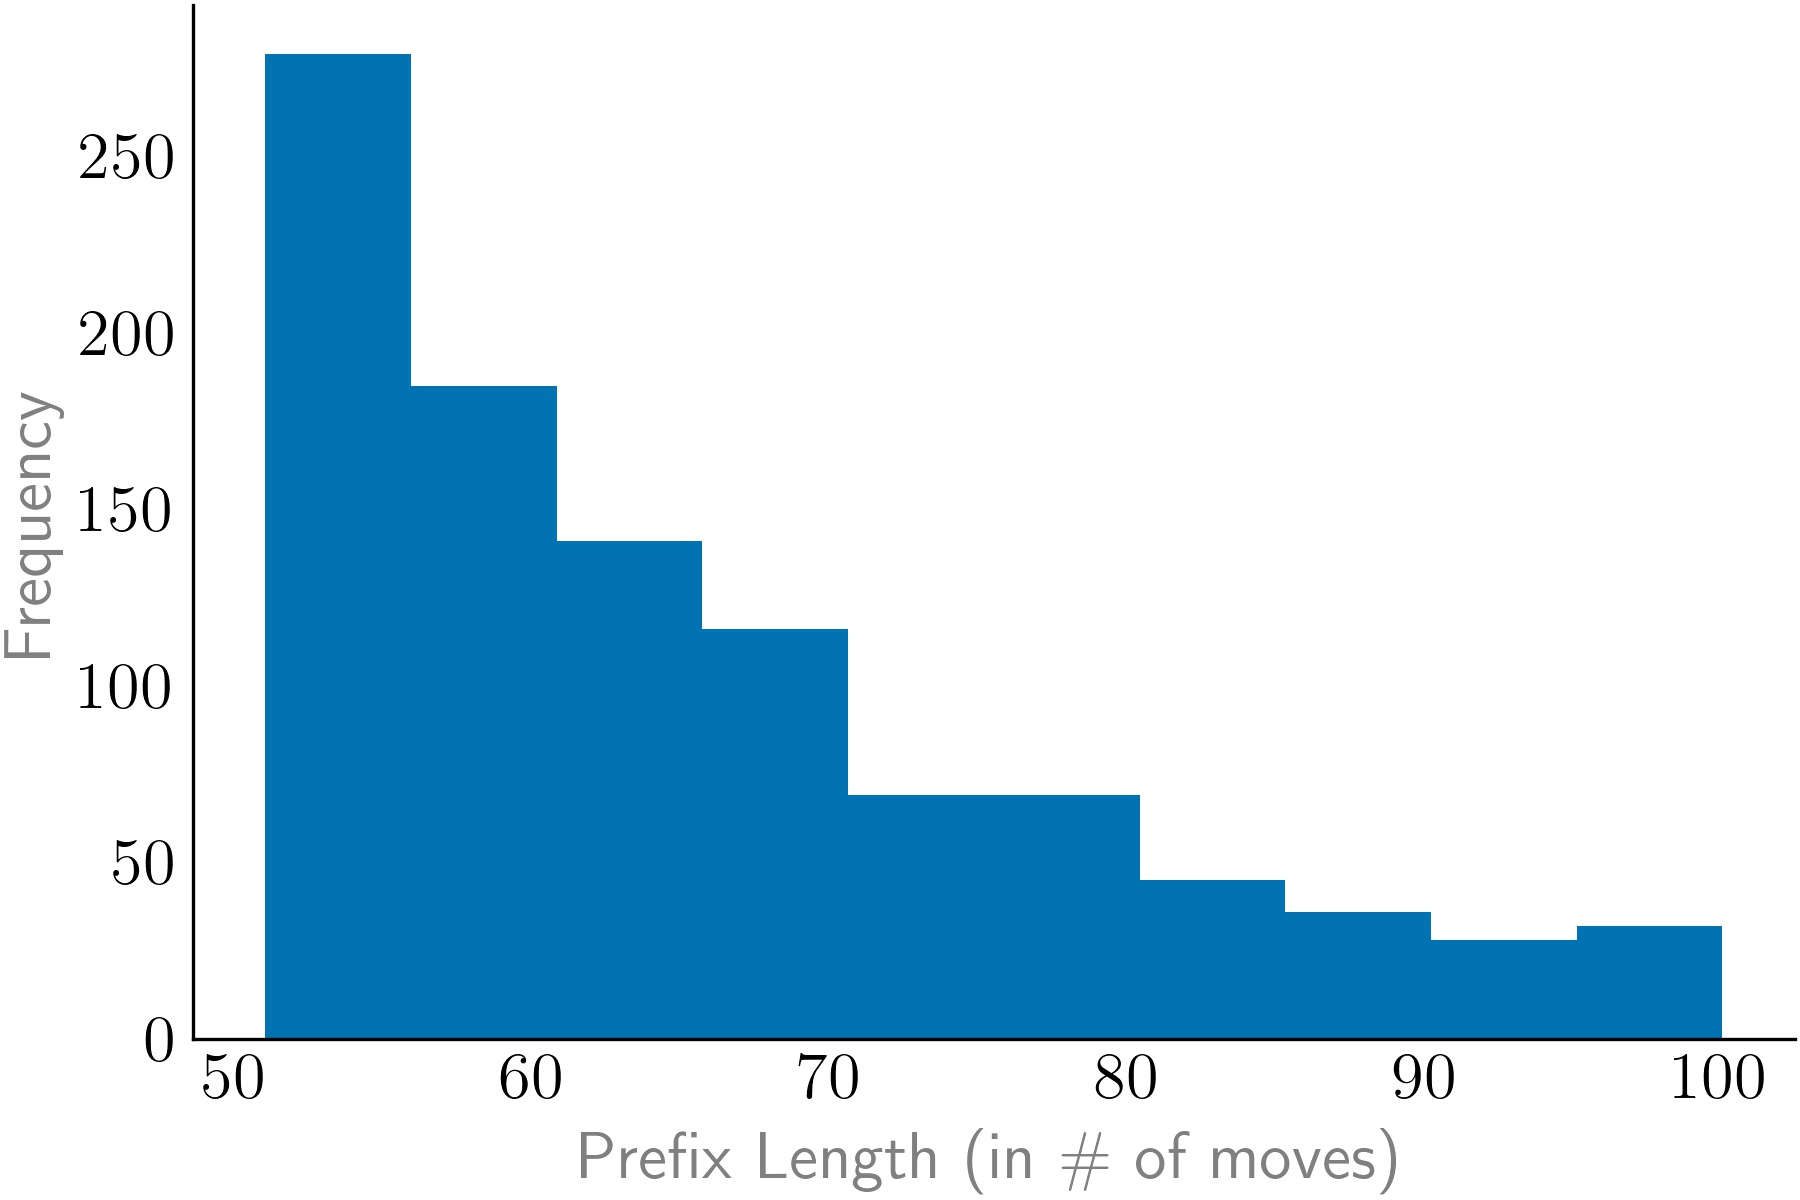
\includegraphics[width=0.8\textwidth]{figures/hist_prefix}
			\vspace{-0.1in}
			\captionof{figure}{Histogram of prefix lengths of board state prompts.}
			\label{fig:hist_prompt}
		\end{minipage}
		\end{minipage}
\end{figure*}


\section{Data Statistics}
\label{sec:data_stats}
Table~\ref{tab:data_stats} presents the statistics of the language modeling dataset used. The average game length for all splits is around 75 moves.
Figure \ref{fig:hist_len} presents the histogram of lengths of tokenized UCI games in Train-L. 

Table~\ref{tab:probe_data_stats} presents the piece type counts for the different board state prompts. All the prompts have the same game prefix i.e. the previous moves, though, the move prefix is different - starting square of the move is used for the ending square predictions while the piece type used for the move is used for the starting square prediction. As the game prefix is the same, End-Actual and Start-Actual use the same piece type for each prompt. 
For the End-Other task, we pick a random starting square among all starting squares from which a legal move can be made, except the starting square used for the actual move.
For the Start-Other task, we pick a random piece type among all piece types which can be legally moved, except the piece type which is actually moved in the game.
The different strategies for picking the random starting square and random piece type explains the different piece type distributions for End-Other and Start-Other. Figure~\ref{fig:hist_prompt} shows the histogram of length of game prefixes (in number of moves) used in board state prompts.

  




